\documentclass{report}

\usepackage{graphicx} % Required for inserting images
\usepackage{amsmath,amssymb}
\usepackage[ruled,vlined]{algorithm2e}


\usepackage{pgfplots}
\pgfplotsset{compat=1.18} % Use a recent compatibility version
\usetikzlibrary{arrows.meta} % For nicer arrows

\usepackage{tcolorbox}
\tcbuselibrary{theorems, skins}  


\definecolor{maincolor}{HTML}{1E90FF}


\SetKwSty{textcolor{maincolor}}
\SetArgSty{textcolor{maincolor}}
\SetCommentSty{textcolor{maincolor}}


\newtcbtheorem{teorema}{Teorema}%
{colback=maincolor!10!white,
 colframe=maincolor!80!black,
 fonttitle=\bfseries,
 coltitle=black,
 boxrule=0.8pt,
 arc=4pt,
 enhanced}{th}

\begin{document}


\section{Introduzione}

In questo corso andremo a vedere le basi della \textbf{Crittografia moderna}. In primis, dobbiamo capire cosa vuol dire “\textit{Crittografia}”. Partiamo dall’etimologia: dal greco \textbf{\textit{kryptós}} (nascosto) – \textbf{\textit{graphía}} (scrittura). In sostanza, la Crittografia è la disciplina che studia e analizza come inviare e ricevere messaggi \textbf{nascosti}. Con il termine “nascosti” si intende che solo ed esclusivamente la sorgente e il destinatario possono leggere il contenuto del messaggio, mentre qualsiasi altra persona non può.

\begin{figure}[h]
     \centering
    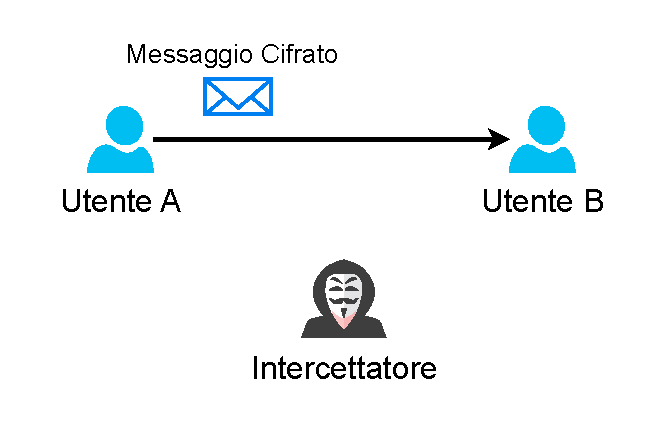
\includegraphics[width=0.6\linewidth]{logos/0_1_cripto.pdf}
\end{figure}

In questa immagine l'utente A manda un messaggio criptato all’utente B; in questo modo solo A e B potranno leggere il contenuto del messaggio, mentre l’intercettatore, anche se riuscisse ad averne una copia, non sarebbe in grado di leggerlo (dato che è criptato).

La crittografia la usiamo tutti i giorni (anche involontariamente) con i nostri dispositivi elettronici. Un esempio è \textbf{WhatsApp}, che tramite una crittografia \textbf{End-to-End} (che avremo tempo di approfondire) permette di inviare messaggi in maniera sicura, in modo che nessun altro (nemmeno WhatsApp stesso!) possa leggere il messaggio che hai mandato al tuo amico. Ha anche utilità nell’autenticazione digitale e nei documenti elettronici: infatti, tutti i sistemi come \textbf{SPID} oppure \textbf{CIE} sfruttano la crittografia per funzionare. La crittografia viene utilizzata anche dalle case produttrici di console (come \textbf{Sony} per la \textbf{PlayStation}) per impedire di crackare le loro console. Di esempi ce ne sono a centinaia e avremo tempo per scoprirli tutti.


Anche se ho elencato molti esempi \textbf{digitali}, la crittografia è una disciplina basata sulla \textbf{matematica}. Infatti, tutti i sistemi crittografici si fondano su prove matematiche (come il \textbf{Logaritmo Discreto} e la \textbf{Fattorizzazione di numeri composti}) per funzionare. Mi piace definire la crittografia come una branca a metà strada tra matematica e informatica, poiché utilizza concetti matematici applicati a contesti informatici.

\newpage

Un altro punto fondamentale da chiarire è che, anche se parleremo di sistemi moderni come \textbf{AES}, \textbf{RSA}, \textbf{Diffie-Hellman} e \textbf{ECC}, inventati tra il 1960 e il 1990 circa, in realtà la crittografia è molto più antica. Già dall’\textbf{Impero Romano} (753 a.C. – 476 d.C.) se ne parlava: chiaramente i sistemi erano molto più semplici di quelli odierni, ma all’epoca servivano per inviare messaggi all’esercito. In questo coro di cifrari "antichi" ne vedremo due, forse i più impattanti nella storia: il \textbf{Cifrario di Cesare}, che possiamo definire il primo sistema crittografico, e la macchina \textbf{Enigma}, che durante la Seconda Guerra Mondiale fu di fondamentale importanza per le truppe dell’Asse; gli alleati, grazie a \textbf{Alan Turing}, riuscirono a decifrarla, aiutando così la loro vittoria.

Fatte tutte le premesse del caso, iniziamo a parlare di crittografia; come prima cosa, vediamo e definiamo tutti i termini utilizzati in questo ambito.


\subsubsection{Cifratura} 

La cifratura di un messaggio è il processo che permette di \textbf{alterare} un messaggio in modo che nessun altro (eccetto chi lo invia e il destinatario) possa leggere il contenuto originario. La cifratura deve avvenire tramite un \textbf{algoritmo di cifratura} e con l’ausilio di una (o più) \textbf{chiavi}.


\begin{figure}[h]
     \centering
    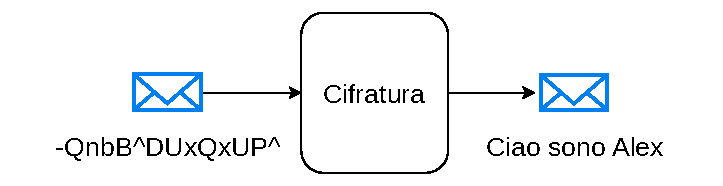
\includegraphics[width=0.8\linewidth]{logos/0_2_cripto.pdf}
\end{figure}

In questo caso, il messaggio "\textbf{Ciao sono Alex}" tramite una cifratura è diventato \textbf{-QnbB\^{}DUxQxUP\^{}}; se qualcuno riuscisse a intercettare il messaggio cifrato, non capirebbe nulla.


\subsubsection{Decifratura} 

La decifratura è il passaggio \textbf{inverso} della cifratura, nel senso che permette di tornare al messaggio originale partendo dal messaggio cifrato. Chiaramente, bisogna usare lo \textbf{stesso algoritmo di cifratura} e, soprattutto, la \textbf{stessa chiave}, che deve essere conosciuta solo da chi invia il messaggio e da chi lo deve ricevere.


\begin{figure}[h]
     \centering
    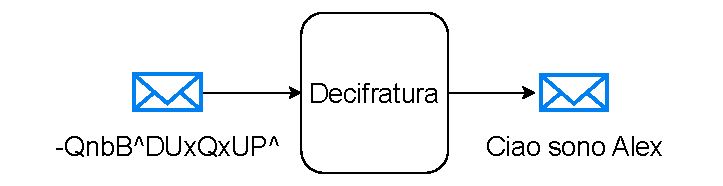
\includegraphics[width=0.8\linewidth]{logos/0_3_cripto.pdf}
\end{figure}


Iniziamo a utilizzare un po' di nozionismo matematico: il meccanismo di cifratura e decifratura può essere paragonato a una \textbf{funzione}, poiché entrambe prendono una variabile in input e restituiscono un valore in output. Possiamo quindi definire la cifratura come


\begin{equation*}
    c = f(m)
\end{equation*}

Dove $c$ è il messaggio cifrato, $m$ è il messaggio originale e $f$ è la “funzione di cifratura”. Dato ciò, la “funzione di decifratura” sarà definita come


\begin{equation*}
    m = f^{-1}(c)
\end{equation*}

Questo può essere dedotto dalla seguente equazione:


\begin{equation*}
    m = f^{-1}(f(m)) 
\end{equation*}

Tranquilli, per ora abbiamo terminato con il nozionismo matematico.


\subsubsection{Chiave} 

Una chiave è una qualsiasi \textbf{stringa} o, più semplicemente, un \textbf{numero}; la caratteristica principale è che una chiave deve \textbf{rimanere privata}, perché permette di cifrare e decifrare i messaggi. Se qualcuno riuscisse a rintracciare la vostra chiave privata, potrebbe leggere tutti i messaggi che inviate e ricevete. L’idea della chiave in crittografia è simile a quella di una \textbf{password}: allo stesso modo, se qualcuno vi ruba la password, può accedere al vostro account. In realtà, la chiave può anche essere qualcosa di più complesso, come un \textbf{punto nel piano cartesiano} (usato nella \textit{Elliptic Curve Cryptography}).

Quindi, per evitare confusione, correggiamo la definizione precedente dicendo che una chiave è un qualsiasi \textbf{dato}, oppure un \textbf{insieme di dati}, che deve rimanere \textbf{segreto}.

In realtà, vedremo verso metà corso che esiste anche una cosiddetta \textbf{chiave pubblica}, ovvero una chiave come quella che abbiamo definito fino a ora, ma che \textbf{chiunque può conoscere}. Se vi sembra strano o controintuitivo, quando lo vedremo tutto sarà chiaro.

\newpage

\subsubsection{Rotto} 

Un sistema crittografico si definisce \textbf{rotto} qualora sia possibile decifrare un messaggio criptato senza conoscere la chiave. Un sistema rotto, chiaramente, non può essere utilizzato, perché chiunque riuscirebbe a decifrare il messaggio. Un esempio di sistema rotto è il \textbf{DES} (che vedremo nel capitolo “Cifrari a Blocchi”). Il DES è stato inventato nel 1976 e, all’inizio, era molto usato; il problema era che utilizzava una chiave a lunghezza fissa: 54 bit. Ad oggi, purtroppo, una chiave a 54 bit è soggetta ad attacchi \textbf{brute-force}\footnote{Attacchi in cui si provano tutte le possibili combinazioni di una chiave; richiedono molto tempo, ma per chiavi molto piccole (come il DES) possono funzionare}, e per questo oggi il DES non può più essere usato per cifrare ed è stato sostituito dall’\textbf{AES}.








\subsection{Principio di Kerckhoffs}

Ora che abbiamo iniziato a familiarizzare con i primi termini della crittografia, possiamo comprendere il principio fondante della disciplina: il \textbf{Principio di Kerckhoffs}.


\begin{teorema}{Principio di Kerckhoffs}{}
La sicurezza di un sistema crittografico deve dipendere unicamente dalla chiave segreta e non dalla segretezza dell’algoritmo stesso.

\end{teorema}

Sostanzialmente, Kerckhoffs afferma che non deve essere segreto \textbf{l’algoritmo di cifratura}; la forza di un sistema crittografico deriva invece dalla difficoltà di romperlo, e non dalla segretezza dell’algoritmo.


Per questo motivo, oggi sappiamo perfettamente quali algoritmi utilizzano i vari siti e le app; non è un rischio conoscere il metodo con cui viene criptato un messaggio, perché la sicurezza risiede nella segretezza della chiave, che, chiaramente, deve rimanere privata. 


Per esempio, secondo Kerckhoffs, se tu e un tuo amico volete creare un sistema per scambiarvi messaggi segreti, non potete semplicemente utilizzare un sistema debole mantenendolo segreto a tutti gli altri; se qualcuno riuscisse a scoprire l’algoritmo, potrebbe leggere tutti i vostri messaggi. i messaggi.



\newpage

\subsection{Il problema dello scambio della Chiave}

Prima di cominciare a parlare della classificazione dei sistemi crittografici, è necessario affrontare il problema dello scambio della chiave. Ripetendo quanto visto finora, la crittografia studia come due utenti possano scambiarsi messaggi in modo che nessun altro ne possa leggere il contenuto. Abbiamo capito che il messaggio viene cifrato e poi decifrato tramite un algoritmo. Inoltre, un algoritmo ha bisogno di una chiave per cifrare i messaggi, e la chiave deve essere posseduta solo da chi invia il messaggio e da chi lo deve ricevere; nessun altro dovrebbe conoscerla, altrimenti anche altri utenti potrebbero decifrare i messaggi. Tuttavia, non abbiamo ancora considerato come i due utenti possano scambiarsi una chiave comune o, comunque, concordare su una chiave da usare nel sistema.


\begin{figure}[h]
    \centering
    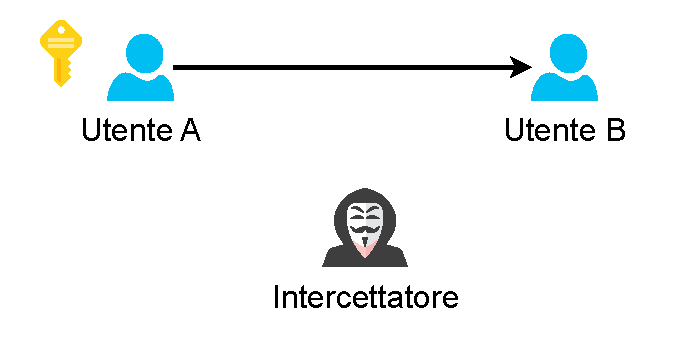
\includegraphics[width=0.6\linewidth]{logos/0_5_cripto.pdf}
\end{figure}

In questa immagine, l’utente A ha generato una chiave da usare per cifrare i messaggi, ma deve trovare un modo per inviarla a B (così che lui possa decifrare i messaggi di A) senza che l’intercettatore riesca a intercettarla. Questo problema è stato risolto tramite i sistemi \textbf{asimmetrici}; come ciò sia possibile lo vedremo quando li studieremo nel dettaglio. Per ora, vi basta sapere che lo scambio della chiave è risolto da questi tipi di sistemi.



\subsection{Le prime Classificazioni}

I sistemi crittografici si dividono in diverse sottocategorie, ognuna con le proprie caratteristiche. Per comprenderle meglio, vediamo subito una mappa riassuntiva di tutte le categorie e poi le commenteremo una ad una. Perciò, ecco a voi la mappa:

\begin{figure}[h]
    \centering
    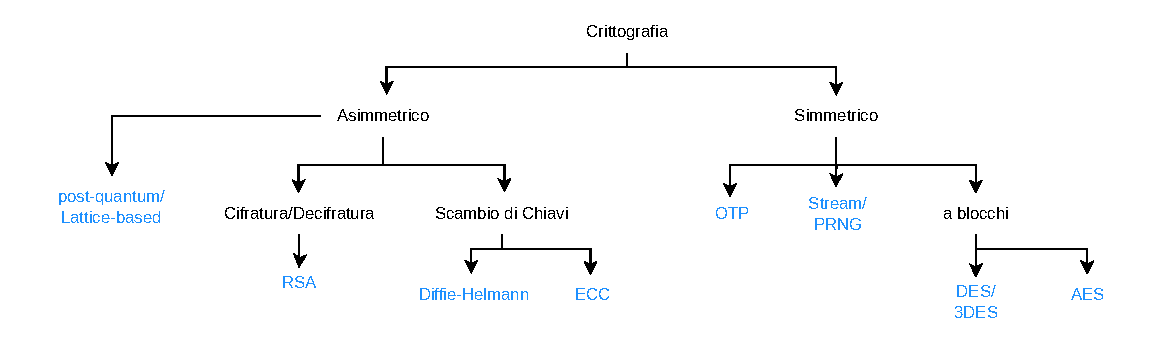
\includegraphics[width=\linewidth]{logos/0_4_cripto.pdf}
\end{figure}





La prima grande distinzione nella crittografia moderna è quella tra sistemi \textbf{simmetrici} e \textbf{asimmetrici}. Un sistema simmetrico utilizza \textbf{una sola chiave}, che deve rimanere sempre privata, mentre i sistemi asimmetrici hanno \textbf{due chiavi: una privata e una pubblica}. I due sistemi sono complementari l’uno all’altro e, ora, vedremo i principali vantaggi e svantaggi di entrambi.

Sistemi Simmetrici:

\begin{itemize}
    \item I sistemi simmetrici sono veloci dal punto di vista computazionale, nel senso che i computer possono eseguire rapidamente gli algoritmi di cifratura e decifratura. 
    
    Questi algoritmi utilizzano combinazioni di operazioni booleane (come lo \textbf{XOR}) e operazioni su matrici, calcoli che i computer sanno eseguire in maniera eccellente. In alcuni casi, è anche possibile parallelizzare alcune fasi per velocizzare ulteriormente il processo.
     
    \item Tuttavia, i sistemi simmetrici non risolvono il problema dello scambio della chiave.
\end{itemize}

Sistemi Asimmetrici:

\begin{itemize}
    \item I sistemi asimmetrici risolvono il problema dello scambio della chiave, nel senso che non è necessario che i due utenti abbiano precedentemente condiviso una chiave segreta.
    \item I sistemi asimmetrici sono più lenti dal punto di vista computazionale, perché devono eseguire operazioni su numeri molto grandi (parliamo di numeri con fino a 600 cifre!).
\end{itemize}


Queste sono, intanto, le prime differenze tra sistemi asimmetrici e simmetrici, e si nota che sono complementari: difficilmente, infatti, nei progetti si utilizza solo uno dei due, perché è preferibile impiegare entrambi. Per esempio, il protocollo \textbf{HTTPS}, che serve per inviare le pagine web in modo cifrato, crea una chiave per un sistema \textbf{simmetrico}, ma la chiave viene cifrata tramite un sistema \textbf{asimmetrico}. In questo modo, i due utenti ottengono la chiave in \textbf{maniera sicura} (perché è stata inviata tramite un sistema asimmetrico), mentre la comunicazione vera e propria utilizza un sistema simmetrico, poiché è più \textbf{veloce}.

\newpage

\subsubsection{Sistemi Simmetrici - OTP}

Tra le due categorie, i sistemi simmetrici sono i primi che vedremo, poiché sono tendenzialmente più semplici. Come si nota dal grafico, i simmetrici si suddividono in altre tre categorie: \textbf{OTP}, \textbf{Stream} e \textbf{a Blocchi}. Il primo che analizzeremo è \textbf{OTP} (\textit{One Time Pad}), l’unico sistema definito \textbf{perfettamente sicuro}, ovvero tale per cui, partendo dal messaggio cifrato senza la chiave, è impossibile risalire al messaggio originale. Tutti gli altri sistemi, se sottoposti ad attacchi \textbf{brute-force}, permettono di risalire al messaggio originale senza la chiave di cifratura. Chiaramente, tali attacchi sono praticamente infattibili perché richiederebbero anni per essere completati; tuttavia, nell’ipotesi di disporre di un computer infinitamente potente, il cifrario OTP sarebbe l’unico \textbf{impossibile} da decifrare senza la chiave.

Dopo questa definizione, potreste pensare che si potrebbe usare sempre e solo l’\textbf{OTP}, ma purtroppo ha un limite che lo rende poco praticabile: è necessario cambiare la chiave dopo ogni cifratura. Infatti, se due messaggi vengono cifrati con la stessa chiave, tramite delle \textbf{criptoanalisi} è possibile risalire sia alla chiave sia ai messaggi originali. Se qualcuno pensasse di generare sempre nuove chiavi, la gestione diventerebbe eccessivamente complessa e insostenibile per la comunicazione.

\subsubsection{Sistemi Simmetrici - PRNG / Stream}

La categoria successiva è quella degli \textbf{Stream}, che però vedremo solo brevemente, poiché non sono molto utilizzati. Gli Stream funzionano generando un \textbf{flusso} (da cui il nome \textit{Stream}) di \textbf{numeri casuali}, che vengono poi utilizzati per cifrare i messaggi tramite l’\textbf{OTP}. Il problema è che la generazione di numeri casuali per i computer è \textbf{impossibile}, poiché i computer sono sistemi \textbf{deterministici}. Per produrre numeri per questo sistema, si utilizzano algoritmi detti \textbf{PRNG} (\textit{Pseudo Random Number Generator}), che cercano di generare numeri apparentemente casuali ma che presentano comunque correlazioni tra loro; con determinati attacchi, è possibile prevedere i numeri successivi dello stream anche senza conoscere la chiave. Per questo motivo, questa tipologia di cifrari oggi non viene quasi mai utilizzata.


\newpage
\subsubsection{Sistemi Simmetrici - A Blocchi}

Finalmente arriviamo ai veri sistemi simmetrici: quelli a blocchi. Questi cifrari sono quelli utilizzati oggigiorno per la loro sicurezza e \textbf{velocità}. I cifrari a blocchi funzionano suddividendo il messaggio in blocchi di n bit. Supponiamo di voler cifrare un messaggio di 120 bit e di avere un cifrario a blocchi che opera su blocchi da 50 bit. In questo caso, il nostro messaggio \textbf{sarà diviso in 3 blocchi:} il primo da 50 bit, il secondo da 50 bit e l’ultimo da 20 bit. Se l’ultimo blocco non raggiunge la dimensione prevista dal cifrario, vengono aggiunti degli zeri (o un qualsiasi \textbf{padding}) in modo che raggiunga la lunghezza di 50 bit.


\begin{figure}[h]
    \centering
    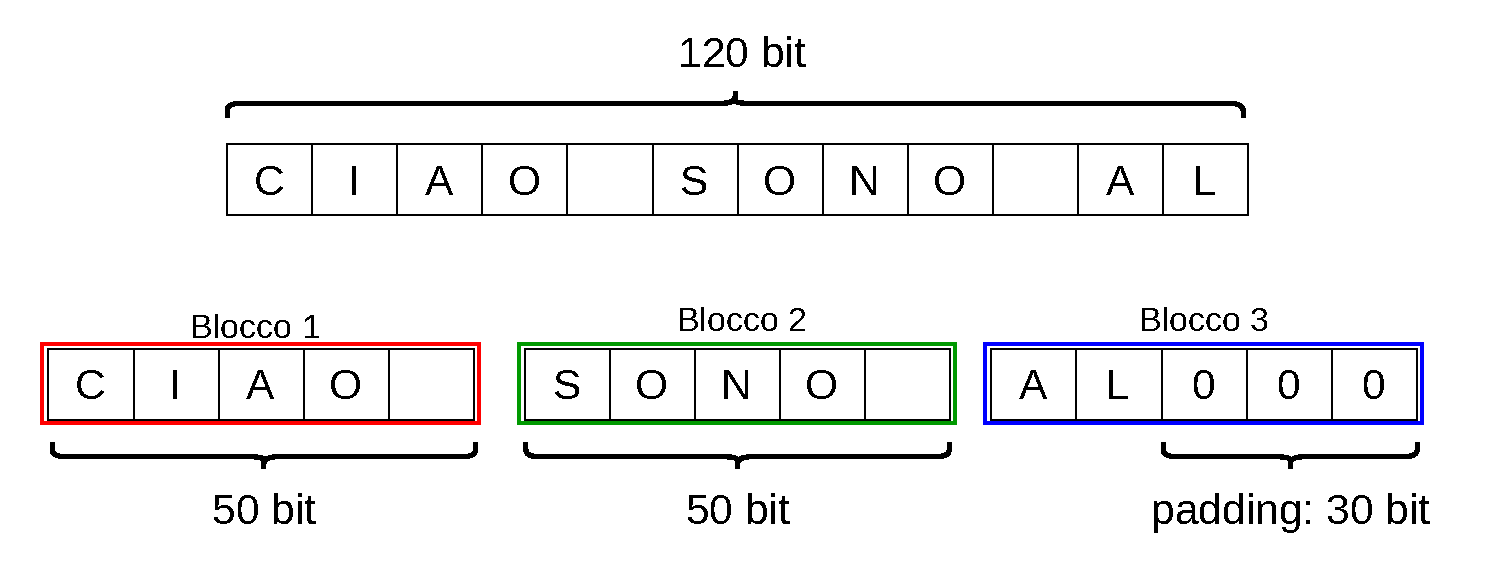
\includegraphics[width=\linewidth]{logos/0_6_cripto.pdf}
\end{figure}



Questo meccanismo di creare blocchi è necessario perché ogni blocco viene poi trasformato in una \textbf{matrice}. Per questo motivo, è importante che ogni blocco abbia una dimensione definita, poiché gli algoritmi sfruttano operazioni su matrici per cifrare il messaggio. Allo stesso modo, il messaggio cifrato sarà anch’esso una matrice della stessa dimensione, che verrà poi riconvertita in messaggio. È importante comprendere che, poiché l’algoritmo cifra un blocco alla volta, lo stesso blocco in input produce sempre lo stesso blocco cifrato. Ciò significa che, se due blocchi all’interno del messaggio originale sono identici, avranno lo stesso blocco cifrato.


\begin{figure}[h]
    \centering
    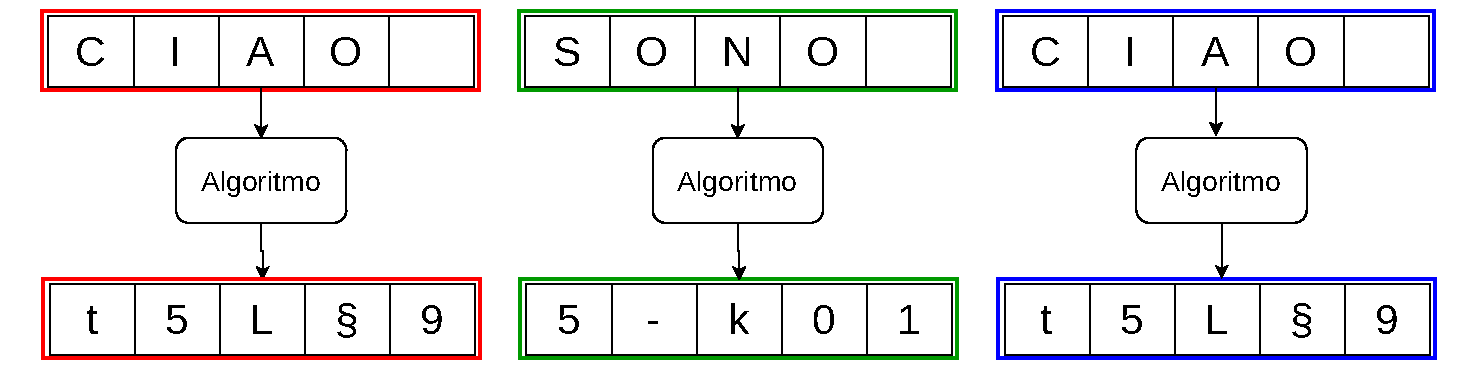
\includegraphics[width=\linewidth]{logos/0_7_cripto.pdf}
\end{figure}

I blocchi cifrati vengono poi riuniti per formare il messaggio cifrato. Per evitare che due blocchi identici producano lo stesso output (cosa che potrebbe aiutare a risalire al messaggio originale), sono stati ideati i \textbf{modi di funzionamento dei cifrari a blocchi}, che vedremo con calma e in dettaglio più avanti.

\newpage

La forza di questi cifrari è che utilizzano soltanto operazioni \textbf{booleane} (\textbf{and}, \textbf{or}, \textbf{xor} e \textbf{not}) e operazioni \textbf{su matrici}, il che li rende molto veloci, poiché queste operazioni sono altamente ottimizzate nei computer odierni.


I principali algoritmi a blocchi sono \textbf{DES} (\textit{Data Encryption Standard}) e \textbf{AES} (\textit{Advanced Encryption Standard}). Il DES nacque nel 1976 e, per i vent’anni successivi, fu lo standard per i cifrari a blocchi. Nel 1999, però, dei ricercatori riuscirono a \textbf{rompere} il cifrario, rendendolo insicuro a causa della breve lunghezza della chiave, che permetteva un attacco brute-force. Al suo posto arrivò \textbf{AES} nel 1998, che ad oggi è ancora considerato un sistema sicuro. Inoltre, fu creato il \textbf{3DES} (\textit{Triple DES}), che consiste nel cifrare un messaggio tre volte con il DES; questo stratagemma permette ancora oggi di usare il DES in forma sicura, anche se oggi si utilizza quasi esclusivamente il 3DES e non più il DES singolo.


\subsubsection{Sistemi Asimmetrici - RSA}

Passando all'altro lato del nostro schema arriviamo ai sistemi \textbf{asimmetrici}. Come abbiamo gia detto, questi sistemi hanno come caratteristica principale che non hanno solamente una chiave ma ne hanno \textbf{una privata e una pubblica}. \text{RSA} (che è l'acronimo dei 3 crittografi che lo hanno inventato) è un algoritmo che permette di creare le due chiavi in maniera sicura, e permette anche ci \textbf{cifrare e decifrare} (cosa che negli algoritmi a \textbf{Scambi di chiave} non è contemplata). RSA sfrtutta la difficoltà di \textbf{Fattorizzare numeri grandi} (che come dicevamo stiamo parlando di numeri a 600 cifre circa). Infatti ad oggi, l'unico modo che abbiamo per fattorizzare un numero è provare a dividere tutti i numeri minori di esso. Quindi per i computer odierni non è sostenibile un calcolo così impegnativo.  

\vspace{0.5cm}


\begin{algorithm}[H]
\caption{Fattorizzazione di un numero $n$}
\KwIn{$n$}
\KwOut{$list$}
$list \gets []$\;
\For{$k \gets 2$ \KwTo $n-1$}{
  \If{$n \bmod k = 0$}{
    $list.append(k)$\;
  }
}
\Return $list$\;
\end{algorithm}


\newpage

\subsubsection{Sistemi Asimmetrici - Scambio di Chiavi}
Tra gli algoritmi asimmetrici abbiamo anche quelli che io ho chiamato \textbf{Scambio di Chiave}, i quali si occupano esclusivamente di \textbf{generare una chiave condivisa tra due utenti}, che poi sarà utilizzata con un algoritmo simmetrico come l'\textbf{AES} o il \textbf{DES}. Questo approccio consente di combinare i vantaggi dei sistemi simmetrici (\textbf{velocità}) con quelli dei sistemi asimmetrici (\textbf{sicurezza}).


Tra questi algoritmi, i due principali sono: \textbf{Diffie-Hellman} (dal nome dei ricercatori che lo hanno inventato) e \textbf{ECC} (\textit{Elliptic Curve Cryptography}). Diffie-Hellman, come vedremo, è molto semplice e sfrutta un meccanismo di potenze e moduli, mentre ECC è più particolare: utilizza infatti una curva ellittica definita da un’equazione del tipo seguente:


\begin{equation*}
    y^2 = x^3 + ax + b    
\end{equation*}

che ha come grafico:


\begin{figure}[h!]
\centering
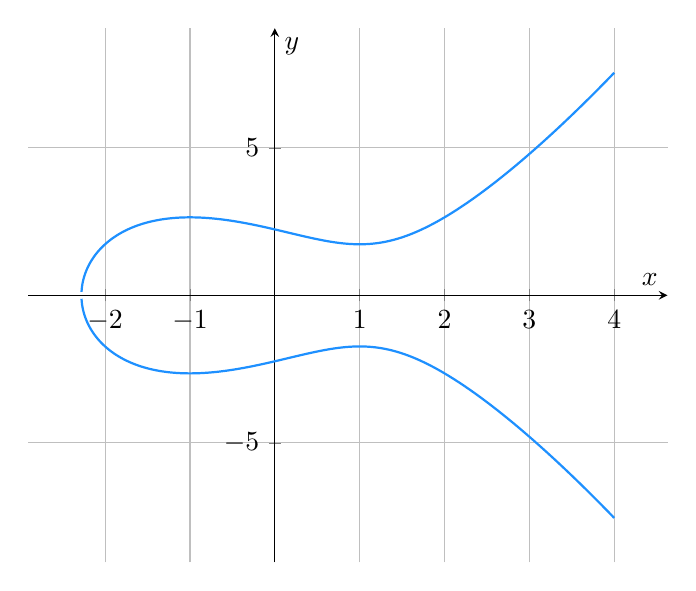
\begin{tikzpicture}
\begin{axis}[
    axis lines=middle, % Axes pass through the origin
    xlabel=$x$,
    ylabel=$y$,
    grid=both,
    enlargelimits=0.1, % Add some padding
    domain=-3:4,    % x-range for the plot
    samples=1300,      % Number of points (for a smooth curve)
    smooth,           % Makes the line smoother
    width=0.8\textwidth
]
% Plot the top half of the curve
\addplot[maincolor, thick] {sqrt(x^3 - 3*x + 5)};

% Plot the bottom half of the curve
\addplot[maincolor, thick] {-sqrt(x^3 - 3*x + 5)};

\end{axis}
\end{tikzpicture}
\end{figure}

L'idea alla base di ECC è quella di \textbf{modulare la curva secondo un numero primo $p$} e di scegliere un punto casuale su di essa, sul quale eseguire una particolare operazione, la \textbf{somma tra punti}, che vedremo con calma, poiché risulta particolarmente complessa.

Ad ogni modo, sia Diffie-Hellman che ECC sfruttano la difficoltà di calcolare il \textbf{logaritmo discreto}. In altre parole, per noi e per i computer è semplice risolvere la seguente equazione:

\begin{equation*}
    2 ^ x = 9
\end{equation*}

Infatti, per risolverlo basta calcolare il logaritmo.

\begin{equation*}
    x = log _ {2} 9
\end{equation*}

\newpage

Il discorso cambia però quando applichiamo questo ragionamento ai moduli (che vedremo meglio in seguito; se non li avete mai visti, potete saltare al prossimo paragrafo). Infatti, se consideriamo un' equazione del genere:

\begin{equation*}
    2 ^ x \equiv 9 \mod 17
\end{equation*}


È complicatissimo risolverla, perché non è più possibile applicare il logaritmo a causa del modulo. Come per la fattorizzazione, ad oggi non esistono algoritmi che permettano di risolvere queste equazioni in tempi ragionevoli.


\subsubsection{Post-Quantum}
Ultimo appunto prima di partire con i cifrari antichi: voglio fare una piccola introduzione sui \textbf{Cifrari Post-Quantum}, perché gli algoritmi \textbf{RSA}, \textbf{Diffie-Hellman} e \textbf{ECC} sono attualmente molto difficili da rompere con i computer moderni, ma è possibile che, con i computer \textbf{quantistici}, possano essere violati anche in pochi secondi. Infatti, i computer quantistici sono particolarmente adatti a risolvere problemi su cui si basano questi algoritmi: ad esempio, possono fattorizzare numeri enormi o calcolare il logaritmo discreto in tempi brevissimi.

Tuttavia, ad oggi i computer quantistici sono ancora in fase di sviluppo e c’è ancora molta strada da fare: per esempio, il numero più grande mai fattorizzato con un computer quantistico è \textbf{21}. Non si può sapere come saranno i computer quantistici in futuro; per questo motivo, i maggiori ricercatori stanno lavorando per creare nuovi cifrari \textbf{difficili da rompere anche per computer quantistici}.

Tra questi, quelli che stanno ricevendo maggiore attenzione dalla comunità scientifica sono i \textbf{Lattice-Based}. Si tratta di algoritmi che sfruttano i \textbf{reticoli} (in inglese \textit{Lattice}), ovvero "piani cartesiani" a n dimensioni, ad esempio $\mathbb{Z} ^ n$.

Si possono generare dei vettori linearmente indipendenti a $n$ dimensioni. A partire da questi, è possibile definire un punto e determinare il percorso più semplice per raggiungerlo usando i nuovi vettori. Ad ogni modo, questi cifrari sono particolarmente complessi, ma rappresentano anche il futuro della crittografia. Per questo motivo, in questo corso non li tratteremo, ma consiglio a tutti di studiarli autonomamente.


\end{document}